%!TEX root = ../../main.tex

\section{General framework}
    We propose a framework for cross-view action recognition as illustrated in Figure \ref{fig:frw}. It composes of two phases: training phase and recognition phase. 
    \begin{itemize}
        \item \textbf{Training phase}: Suppose we have $v$ views. The training phase consists of three main steps: 
        \begin{enumerate}
            \item \textit{Feature extraction at separated view}: All training samples from each separated view will be passed though a feature extraction step. Different deep techniques will be investigated, including 2D CNNs based feature extraction combined with aggregation techniques and 3D CNNs based feature extraction, to output the final descriptor for each video sample. Let's call the features extracted at this step as features at single views or separated view features. 
            \item \textit{Common space construction}: This step builds a common feature space so that samples belonging to the same class will be close to each other even they are captured from different viewpoints. It takes all separated view features extracted from training set from the previous step and find a set of $v$ linear transformations $({\omega}_1, {\omega}_2, ..., {\omega}_v)$ that minimize within-class variation while maximizing between-class variation of features in the projected space (common space). 
            \item \textit{Training classifier}: Once $v$ transformations have been computed, the projected features in the common space of each view will be utilized to train a simple predictive model $F$ (i.e. kNN).
        \end{enumerate}
        \item \textbf{Recognition phase}. Multi-view recognition consists of two following steps:
        \begin{enumerate}
            \item \textit{Feature extraction} Features of the testing sample $x_j$ from the view $V_j$ are extracted. This feature will be projected in the pre-built common space by the corresponding transformation ${\omega}_j$. The projected feature is denoted as $y_j = {\omega}^T_j*x_j$.
            \item \textit{Class prediction}: The projected feature $y_j$ will be passed into the classifier $F(y_j)$ that outputs the label of action.
        \end{enumerate}
    \end{itemize}
    \begin{figure}[htbp]
        \centering
        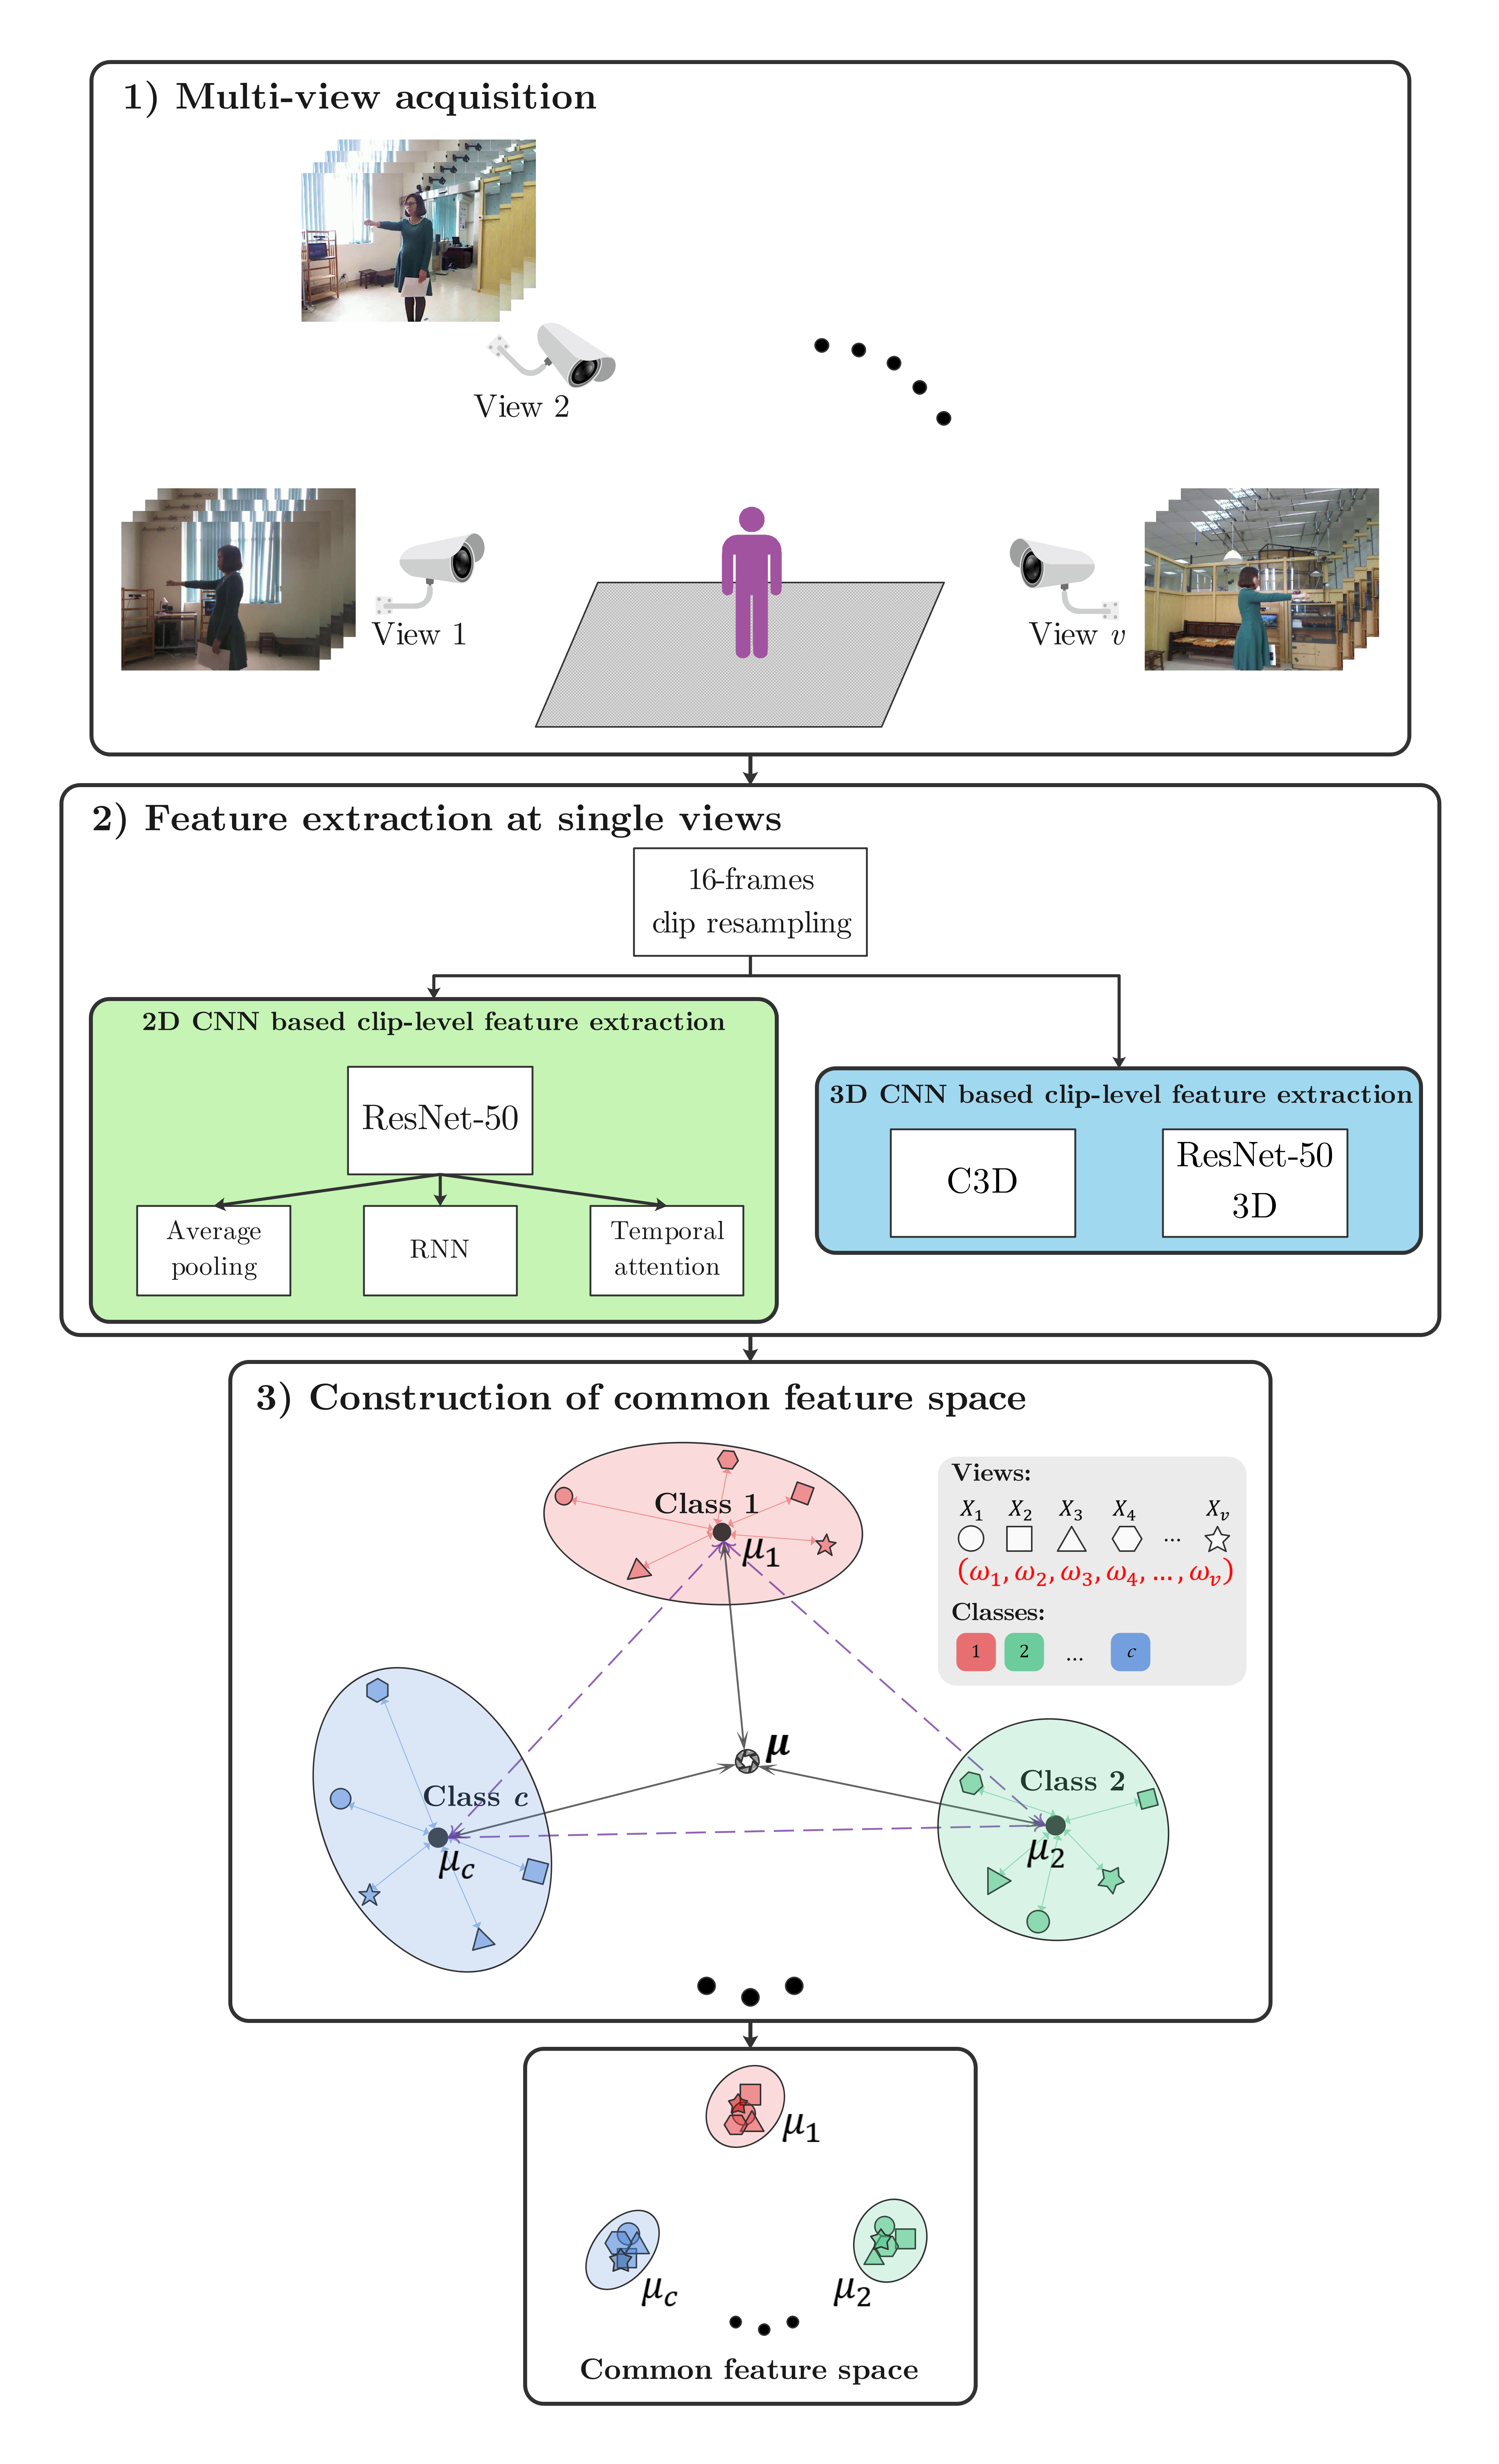
\includegraphics[width=0.82\linewidth]{Figs/Framework.png}
        \caption{Proposed framework for building common feature space with pairwise-covariance multi-view discriminant analysis (pc-MvDA)}
        %\vspace{-0.3cm}
        \label{fig:frw}
    \end{figure}
    %In the following, I will detail the step of feature extraction at separated view in subsection \ref{sub:private}, the step of building the common feature space in subsection \ref{sub:common}. 
